\documentclass[12pt]{article}
\usepackage[utf8]{inputenc}
\usepackage[T1]{fontenc}
\usepackage{amsmath, amsfonts, amssymb}
\usepackage{graphicx}
\usepackage{geometry}
\usepackage{float}
\geometry{a4paper, margin=0.5in}

\title{Fundamentals of 3D Computer Graphics: The Rendering Pipeline}
\author{Huyen Nguyen}
\date{January 2025}

\begin{document}

\maketitle

\section{Introduction: The Graphics Pipeline}

The process of generating a 2D image from a 3D scene is a fundamental task in computer graphics. This process is typically broken down into a series of sequential stages, collectively known as the \textbf{graphics pipeline} [1-7]. Understanding this pipeline is crucial for comprehending how 3D models are brought to life on our screens. These lecture notes will guide you through the initial stages of this pipeline, focusing on how 3D geometry is prepared for the subsequent rendering processes.

The core stages we will cover initially are:

\begin{itemize}
    \item \textbf{Modelling Transformations}: Manipulating objects within their local coordinate systems and placing them in the scene.
    \item \textbf{Change of Coordinates}: Transforming objects between different reference frames.
    \item \textbf{Projection}: Mapping the 3D scene onto a 2D image plane.
    \item \textbf{Clipping}: Removing parts of objects that fall outside the camera's view.
\end{itemize}

These steps lay the groundwork for later stages such as illumination (determining the colour of surfaces), rasterisation (converting 2D primitives into pixels), and visibility determination (deciding which objects are visible).

\section{Modelling Transformations}

Before we can project and render a 3D scene, we need to be able to define and manipulate the objects within it. \textbf{Modelling transformations} allow us to position, orient, and deform objects in 3D space [2, 3]. These transformations are typically represented using $4 \times 4$ matrices, enabling us to apply them to vertices (represented as homogeneous coordinates).

Common elementary transformations include:

\begin{itemize}
    \item \textbf{Translation}: Moving an object along one or more axes. A translation matrix by $(t_x, t_y, t_z)$ is given by:
    \[
    T(t_x, t_y, t_z) = \begin{pmatrix} 1 & 0 & 0 & t_x \\ 0 & 1 & 0 & t_y \\ 0 & 0 & 1 & t_z \\ 0 & 0 & 0 & 1 \end{pmatrix}
    \]
    \item \textbf{Rotation}: Rotating an object around a specified axis. Rotation matrices around the X, Y, and Z axes by an angle $\theta$ are:
    \[
    R_x(\theta) = \begin{pmatrix} 1 & 0 & 0 & 0 \\ 0 & \cos\theta & -\sin\theta & 0 \\ 0 & \sin\theta & \cos\theta & 0 \\ 0 & 0 & 0 & 1 \end{pmatrix}, \quad
    R_y(\theta) = \begin{pmatrix} \cos\theta & 0 & \sin\theta & 0 \\ 0 & 1 & 0 & 0 \\ -\sin\theta & 0 & \cos\theta & 0 \\ 0 & 0 & 0 & 1 \end{pmatrix}, \quad
    R_z(\theta) = \begin{pmatrix} \cos\theta & -\sin\theta & 0 & 0 \\ \sin\theta & \cos\theta & 0 & 0 \\ 0 & 0 & 1 & 0 \\ 0 & 0 & 0 & 1 \end{pmatrix}
    \]
    \item \textbf{Scaling}: Changing the size of an object along one or more axes. A scaling matrix by $(s_x, s_y, s_z)$ is:
    \[
    S(s_x, s_y, s_z) = \begin{pmatrix} s_x & 0 & 0 & 0 \\ 0 & s_y & 0 & 0 \\ 0 & 0 & s_z & 0 \\ 0 & 0 & 0 & 1 \end{pmatrix}
    \]
    \item \textbf{Shearing (Glissement)}: Distorting the shape of an object by shifting points parallel to a plane [8]. For instance, a shear parallel to the x-axis with a factor $k$ has the matrix:
    \[
    \begin{pmatrix} 1 & 0 & 0 & 0 \\ 0 & 1 & k & 0 \\ 0 & 0 & 1 & 0 \\ 0 & 0 & 0 & 1 \end{pmatrix} \quad \text{(Shear parallel to y with respect to z)}
    \]
    The source [8] also provides the matrix for a shear parallel to x with a ratio $k$ and a baseline $y = y_{ref}$:
    \[
    \begin{pmatrix} 1 & 0 & 0 & 0 \\ k & 1 & 0 & 0 \\ 0 & 0 & 1 & 0 \\ -k y_{ref} & 0 & 0 & 1 \end{pmatrix}
    \]

    Here are an example of a standart shear:
    \begin{figure}[H]
        \centering
        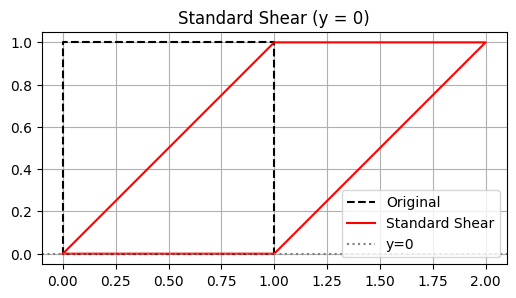
\includegraphics[width=0.4\textwidth]{figures/standart_shear.png}
        \caption{Standart shear}
        \label{fig:standart_shear}
    \end{figure}

    And a shear with a baseline:
    \begin{figure}[H]
        \centering
        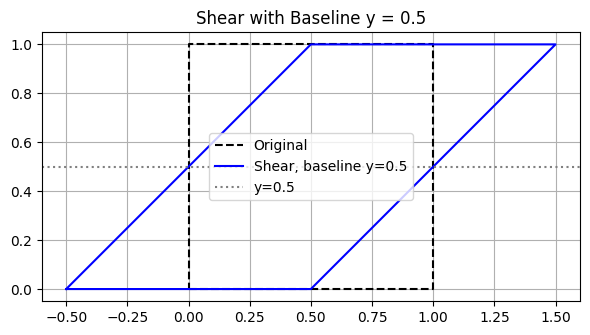
\includegraphics[width=0.4\textwidth]{figures/shear_with_baseline.png}
        \caption{Shear with a baseline}
        \label{fig:baseline_shear}
    \end{figure}
\end{itemize}

\subsection{Composition of Transformations}

Multiple transformations can be combined into a single transformation matrix by multiplying their individual matrices together [1]. The order of multiplication is crucial. If we apply transformation $M$ followed by $M'$, the resulting transformation $M' \cdot M$ is applied to a point $p$ as $p'' = M' \cdot (M \cdot p) = (M' \cdot M) \cdot p$. Importantly, the order of application reads from right to left [1].

To perform a transformation around an arbitrary point $P$, we use a sequence of transformations [1, 9, 10]:

\begin{enumerate}
    \item Translate the object so that the point $P$ coincides with the origin of the scene's coordinate system ($T_{P \rightarrow O}$).
    \item Perform the desired transformation (e.g., rotation $R$).
    \item Translate the object back to its original position by applying the inverse translation ($T_{O \rightarrow P}$).
\end{enumerate}
The combined transformation matrix $M$ is then $M = T_{O \rightarrow P} \cdot R \cdot T_{P \rightarrow O}$. For a rotation $R(\theta_z)$ around the z-axis passing through a point $P(T_x, T_y, T_z)$, the matrix would be:
\[
M = \begin{pmatrix} 1 & 0 & 0 & T_x \\ 0 & 1 & 0 & T_y \\ 0 & 0 & 1 & T_z \\ 0 & 0 & 0 & 1 \end{pmatrix} \cdot \begin{pmatrix} \cos\theta_z & -\sin\theta_z & 0 & 0 \\ \sin\theta_z & \cos\theta_z & 0 & 0 \\ 0 & 0 & 1 & 0 \\ 0 & 0 & 0 & 1 \end{pmatrix} \cdot \begin{pmatrix} 1 & 0 & 0 & -T_x \\ 0 & 1 & 0 & -T_y \\ 0 & 0 & 1 & -T_z \\ 0 & 0 & 0 & 1 \end{pmatrix}
\]
The expanded form of this composition is shown in [10].

\subsection{Hierarchical Modelling (Scene Graphs)}

Complex objects and scenes are often composed of simpler parts, arranged in a hierarchy [11, 12]. \textbf{Hierarchical modelling} uses these relationships to define objects. A \textbf{scene graph} is a data structure, often a Directed Acyclic Graph (DAG), that represents this hierarchy [11]. Each node in the graph can represent an object or a part of an object, and the edges represent the transformations applied to its children relative to its parent.

This approach simplifies the application of transformations. When a transformation is applied to a parent node, all its descendants are also transformed accordingly. This is useful for modelling articulated objects (e.g., a robot arm) or complex structures (e.g., a building with multiple floors and rooms).

\textbf{Instancing} is a technique used within scene graphs to efficiently represent multiple copies of the same object [12]. Instead of storing the geometry of the object multiple times, we can have multiple "pointer" nodes in the scene graph that all refer to the same underlying geometry, each with its own transformation.

\section{Change of Coordinates}

As objects move through the graphics pipeline, their coordinates are transformed from one reference frame (or coordinate system) to another [3, 13]. This is essential for placing objects in the scene, positioning the camera, and finally projecting the scene onto the 2D screen. Key coordinate systems include:

\begin{itemize}
    \item \textbf{Object Space (Model Space)}: The local coordinate system in which an individual object is defined.
    \item \textbf{World Space (Scene Space)}: A global coordinate system in which all objects in the scene are placed and positioned. Modelling transformations are used to move objects from object space to world space.
    \item \textbf{Camera Space (View Space)}: The coordinate system relative to the camera. The camera is typically located at the origin, looking along the negative Z-axis, with the Y-axis pointing upwards and the X-axis to the right. A \textbf{view transformation} (often a composition of a rotation and a translation) transforms the world space into camera space.
\end{itemize}

The transformation from one coordinate system to another can be represented by a matrix multiplication [13]. For example, to transform a point from coordinate system $R_1$ to $R_2$, we can use a transformation matrix $M'_{R_1 \rightarrow R_2}$ such that $p_{R_2} = M'_{R_1 \rightarrow R_2} \cdot p_{R_1}$. This matrix encapsulates the rotation and translation needed to align $R_1$ with $R_2$.

\section{Projection}

\textbf{Projection} is the process of mapping the 3D scene, as viewed from the camera, onto a 2D image plane (the screen) [3, 14, 15]. This reduces the dimensionality of the scene from 3D to 2D [16]. Projections are formed by the intersection of \textbf{projectors} (lines) emanating from a \textbf{centre of projection (CP)} and passing through each point of an object, with the \textbf{projection plane} [17-19].

There are two main types of geometric projections [19, 20]:

\begin{itemize}
    \item \textbf{Parallel Projection}: The CP is at infinity, and all projectors are parallel [19, 21]. Parallel projections preserve parallel lines and ratios of distances along a given direction [22].
    \begin{itemize}
        \item \textbf{Orthographic Projection}: The direction of projection is perpendicular to the projection plane [19, 21, 23]. This is equivalent to discarding one of the coordinate dimensions [23, 24]. For example, projecting onto the XY-plane involves setting the z-coordinate to zero. The projection matrices for orthographic views (top, front, side) are given in [25-27].
        \item \textbf{Oblique Projection}: The direction of projection is not perpendicular to the projection plane [19, 21, 28].
    \end{itemize}
    \item \textbf{Perspective Projection}: The CP is located at a finite point in 3D space, causing projectors to converge at this point [19, 29-32]. Perspective projection simulates how objects appear in the real world, with objects appearing smaller the farther they are from the camera [33-36]. Parallel lines that are not parallel to the projection plane converge at a \textbf{vanishing point} [33, 37, 38]. Perspective projections do not preserve parallelism or exact measurements [33]. The calculation for a single-point perspective projection is shown in [37, 39]. The perspective projection matrix transforms a point $(x, y, z, 1)$ to $(fx/(f-z), fy/(f-z), f/(f-z), 1)$, which after the perspective division (dividing by the w-component) becomes $(x f/(f-z), y f/(f-z), f/(f-z))$ [5, 37, 39-43]. The matrix form involves a $-z$ term in the w-component, leading to the perspective division.
\end{itemize}

\section{View Frustum and Clipping Planes}

The \textbf{view frustum} is the 3D region of space that is visible to the camera. It is typically defined by six planes: near, far, left, right, top, and bottom [44, 45]. The \textbf{near plane} and \textbf{far plane} are parallel to the projection plane and define the range of depths that will be rendered [44]. Objects outside this depth range are not considered. These clipping planes are important for managing the finite precision of the \textbf{depth buffer (z-buffer)} [44, 45]. Values near zero in floating-point numbers have higher precision, so limiting the range between the near and far planes helps in accurately resolving depth comparisons.

Before the final 2D projection, the view frustum is often transformed into a canonical view volume, a cube in \textbf{Normalised Device Coordinates (NDC)} ranging from $[-1, 1]$ in all three dimensions [45, 46]. This normalisation simplifies subsequent clipping operations. The transformation to NDC involves scaling and translation, and for perspective projection, a perspective transformation is applied to account for the foreshortening effect [47-49].

\section{Clipping}

\textbf{Clipping} is the process of discarding primitives (or parts of primitives) that lie outside the viewing volume defined by the view frustum (after projection and transformation to NDC) [4, 50]. This step is crucial for efficiency, as it avoids unnecessary processing (rasterisation and shading) of geometry that is not visible on the screen.

Clipping can be performed against each of the six planes of the view frustum. Different algorithms exist for clipping different types of primitives [51]:

\begin{itemize}
    \item \textbf{Point Clipping}: A point $(x, y, z)$ is inside the viewing volume if it satisfies the conditions $x_{min} \le x \le x_{max}$, $y_{min} \le y \le y_{max}$, and $z_{near} \le z \le z_{far}$ (in camera space or NDC) [12, 51].
    \item \textbf{Line Segment Clipping}: Determining which parts of a line segment lie inside the viewing volume. Algorithms like \textbf{Cohen-Sutherland} [51-54] and \textbf{Liang-Barsky} [51, 55-57] efficiently determine whether a line segment is completely inside, completely outside, or partially inside the clip volume. Cohen-Sutherland uses outcodes to quickly identify trivial cases, while Liang-Barsky uses the parametric form of the line segment. Extension to 3D clipping involves 6-bit outcodes [55].
    \item \textbf{Polygon Clipping}: Clipping polygons against the boundaries of the viewing volume. The \textbf{Sutherland-Hodgeman} algorithm [51, 58] processes a polygon edge by edge against each clip plane. For each edge of the clip volume, it examines the vertices of the polygon and determines which vertices and intersection points should be kept to form the clipped polygon.
\end{itemize}

\section{Rasterisation}

\textbf{Rasterisation} (or scan conversion) is the process of taking the 2D projected primitives (points, lines, and polygons) and determining which pixels on the screen they cover [3, 5, 41]. It involves sampling the primitives at discrete pixel locations and interpolating vertex attributes (such as colour and depth) across the primitive.

\subsection{Line Drawing}

Algorithms like \textbf{Bresenham's line algorithm} [42, 46, 48, 49, 59-67] are efficient methods for determining which pixels lie on or close to a straight line segment. These algorithms use integer arithmetic to make fast decisions about which pixel to activate at each step. The basic idea is to keep track of an error term that represents the distance between the ideal line and the chosen pixel, and to make incremental decisions to minimise this error. Various optimisations to Bresenham's algorithm exist to eliminate floating-point operations and divisions [49, 63-66].

\subsection{Polygon Filling}

Once a polygon is projected onto the 2D screen, we need to fill its interior with colour. The \textbf{scan-line algorithm} [29, 68-72] is a common approach. It works by iterating through each scan line (row of pixels) that intersects the polygon. For each scan line, it finds the intersection points of the scan line with the edges of the polygon, sorts these intersection points by their x-coordinate, and then fills the pixels between pairs of consecutive intersection points. A parity rule is often used to determine whether a pixel is inside or outside the polygon [69, 72].

Another approach for filling regions is the \textbf{seed filling} or \textbf{flood fill algorithm} [73-75]. Starting from an interior pixel (the seed), the algorithm recursively fills adjacent pixels that have the same original colour (or satisfy a certain condition) until a boundary of a different colour is reached.

\subsection{Anti-aliasing}

The discretisation inherent in the rasterisation process can lead to visual artifacts like jagged edges (aliasing) [31, 32, 50, 53, 54, 67, 76, 77]. \textbf{Anti-aliasing} techniques are used to reduce these artifacts. Common methods include:

\begin{itemize}
    \item \textbf{Supersampling}: Rendering the scene at a higher resolution than the target resolution and then downsampling (filtering) the result to produce a smoother image [34-36, 38, 41, 43, 46, 62, 78, 79]. Different sampling patterns (deterministic, random, jittered) and filter shapes can be used [35].
    \item \textbf{Coverage-based methods}: Determining the fraction of a pixel that is covered by the primitive and using this coverage as an alpha value to blend the object's colour with the background [49, 63, 80-82]. Algorithms like \textbf{Gupta-Sproull} [81, 82] adjust the intensity of pixels near the line based on their distance from it.
\end{itemize}

\section{Illumination (Shading)}

Once the 2D primitives are rasterised, the next stage is \textbf{illumination} or \textbf{shading}, which determines the colour of each pixel based on the lighting in the scene, the material properties of the objects, and the surface normals [2, 83, 84]. This topic will be covered in detail in subsequent lectures, but it's important to understand that the geometric information established in the earlier stages (transformations, projections, and surface normals) is crucial for these calculations.

Different illumination models (e.g., ambient, diffuse, specular, Blinn-Phong) and shading techniques (e.g., flat shading, Gouraud shading, Phong shading) are used to achieve various visual effects [14-16, 18, 20, 21, 23, 26, 27, 29, 30, 85-100]. \textbf{Texture mapping} is also used to add detail and visual complexity to surfaces by applying images to them [28, 31, 32, 34, 101, 102].

\section{Visibility / Rendering}

The final stage we will briefly touch upon is \textbf{visibility determination} or \textbf{rendering}, which deals with deciding which objects (or parts of objects) are visible to the camera and should be drawn [2, 6, 88]. Several algorithms exist to solve this problem, including:

\begin{itemize}
    \item \textbf{Backface Culling}: Discarding polygons whose normals point away from the camera [103, 104].
    \item \textbf{Painter's Algorithm}: Sorting polygons by depth and drawing them from back to front [68, 104-106].
    \item \textbf{Binary Space Partitioning (BSP) Trees}: Dividing the scene into a hierarchical structure to determine visibility order [68, 105, 107, 108].
    \item \textbf{Warnock's Algorithm}: A recursive subdivision algorithm that divides the screen into smaller quadrants to resolve visibility [69, 105, 109, 110].
    \item \textbf{Scan-line Algorithms}: Extending the scan-line rasterisation to also handle depth information and visibility [7, 73-75, 103, 111].
    \item \textbf{Z-buffer (Depth Buffer) Algorithm}: A widely used image-space algorithm that stores the depth of the closest object at each pixel, allowing for efficient visibility determination without explicit sorting [75, 103, 112-118]. For each pixel covered by a primitive, its depth is compared to the currently stored depth in the z-buffer. If the new depth is closer to the camera, it replaces the stored depth, and the pixel's colour is updated.
\end{itemize}

The choice of visibility algorithm depends on factors such as scene complexity, hardware capabilities, and desired rendering effects [117, 118].

\section{Conclusion}

This lecture has provided an overview of the initial stages of the 3D computer graphics rendering pipeline. We have explored how modelling transformations are used to manipulate objects, how coordinate systems facilitate the representation of the scene from different perspectives, how projection maps the 3D world to a 2D image, and how clipping defines the visible portion of the scene. These fundamental concepts are essential building blocks for understanding the subsequent stages of the pipeline, which deal with determining the appearance of surfaces and ultimately generating the final image. A solid grasp of these geometric transformations is key to appreciating the intricacies of 3D computer graphics.

\end{document}
